% Report of results from Ramsay simulation experiment
% David Lawrence Miller
% d.l.miller@bath.ac.uk

% Started : 8th April 2009

\documentclass[a4paper,10pt]{amsart}

% Load some packages
\usepackage{times, amsmath, amssymb, amsfonts, url, natbib, bm, rotating,multirow,graphicx}

% top matter
\title{Smoothing over irregular shapes using the Schwarz-Christoffel transform}
\author{David Lawrence Miller}
\email{d.l.miller@bath.ac.uk}
\address{Mathematical Sciences, University of Bath, Bath, United Kingdom}

% Shortcuts
% Probability
\newcommand{\prob}[1]{\mathbb{P}\left[ #1 \right]}
% Hovitz-Thompson
\newcommand{\HT}{\hat{\tau}_{HT}}
% Schwarz-Christoffel
\newcommand{\sch}{Schwarz-Christoffel }
% fprime
\newcommand{\fprime}{f^\prime(z)}
% figure reference command
\newcommand{\fig}[1]{\emph{fig.} (\ref{#1})}
% figure reference command (start of sentance
\newcommand{\Fig}[1]{\emph{Fig.} (\ref{#1})}
% equation reference command
\newcommand{\eqn}[1]{\emph{eqn.} (\ref{#1})}
% phi inverse
\newcommand{\phiinv}{\phi^{-1}}
% use other phi
\newcommand{\ophi}{\phi}
\renewcommand{\phi}{\varphi}




\begin{document}

% The abstract
\begin{abstract}
Following on from looking at the Ramsay horseshoe, other polygon mappings are simulated from and transformed with the \sch transform.
\end{abstract}


% New theorem for theorems
\newtheorem{thm}{Theorem}[section]

%New theorem for definitions
\newtheorem{defn}{Definition}[section]

\maketitle



\section{Looking at other domains}

Given the relative success of using the \sch transform on the Ramsay horseshoe, and the relative failure of using it on the alternate Ramsay horseshoe, more conclusive evidence is needed to investigate the properties of the transform and its utility to smoothing over complex regions.

\section{Figure 9}

We first take a look at the polygon shown in \fig{fig9} and map to both the rectangle and the unit disk. Data was then generated from two multivariate Normal distributions which was discretized over a 500 by 500 grid of points. Taking this as truth, samples were taken and a smooth fit using thin plate regression spllines using \texttt{mgcv}.


\begin{figure}
\centering
% trim order l b r t
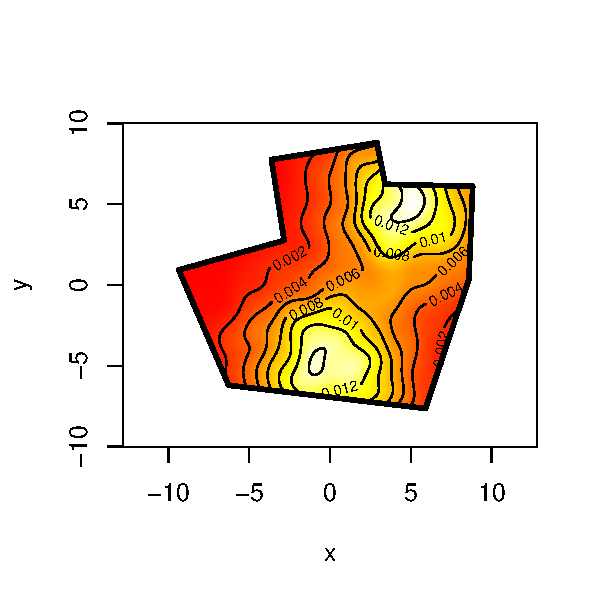
\includegraphics[width=2in]{figs-otherdomains/fig9.png} \\
\caption{The heatmap of the polygon's generated density.}
\label{fig9}
% generated by /phd-smoothing/sc-writeup/figs-otherdomains/fig9.R
\end{figure}

Using the SC Toolbox, the polygon was deformed to both a rectangle and the unit disk. 


Using rectangle and disk mapping. How was the density simulated. Why doesn't it work as well as tprs.


Using the rectangular mapping, vertices chosen (somewhat arbitrarily) to map to those of the rectangle were [NUMBERS] (see [fig].) Fits were found using the trasnformation, thin plate splines and soap at two noise levels ($\sigma^2=0.02$ and $\sigma^2=2$.)

\begin{table}[ht]
\begin{tabular}{c c c}\\
Method & Noise level & MSE \\
\hline
\hline
SC(rect)+tprs & 0.02 & 5.407153e-06\\ 
tprs & 0.02 & 9.257684e-06\\
soap & 0.02 & 1.624942e-06\\
SC(rect)+tprs & 2 & 0.001649676\\
tprs & 2 & 0.001196396\\
soap & 2 & 0.0003585027\\
SC(disk)+tprs & 0.02 & 5.22576e-06\\ 
tprs & 0.02 & 9.155156e-06 \\
soap & 0.02 & 1.580917e-06 \\
SC(disk)+tprs & 2 & 0.001717203 \\
tprs & 2 & 0.002501872 \\
soap & 2 & 0.0002707923 \\
\end{tabular}
\caption{}
\label{}
\end{table}


\begin{figure}
\centering
% trim order l b r t
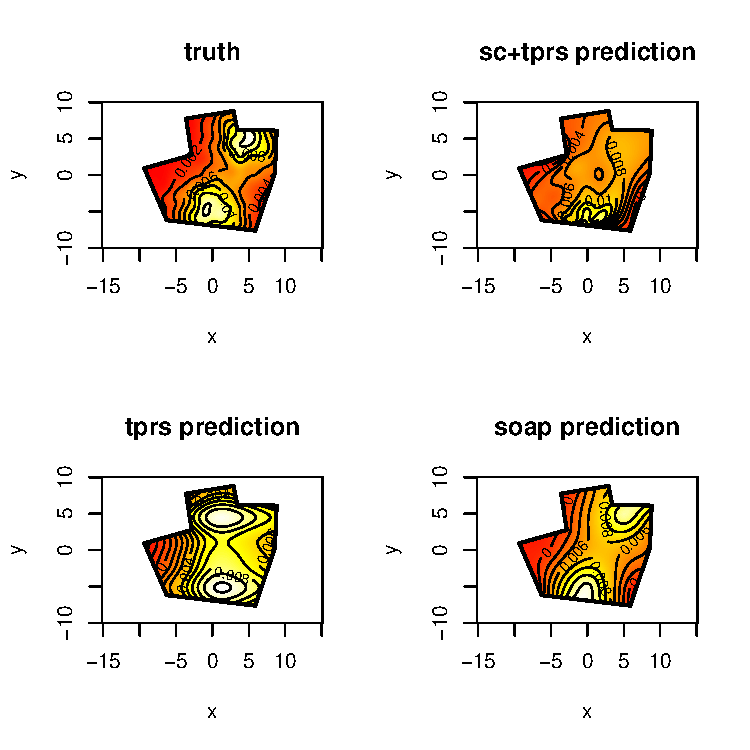
\includegraphics[width=2.5in]{figs-otherdomains/fig9-low-rect.png} \\
\caption{low rect}
\label{fig9-low-rect}
\end{figure}

\begin{figure}
\centering
% trim order l b r t
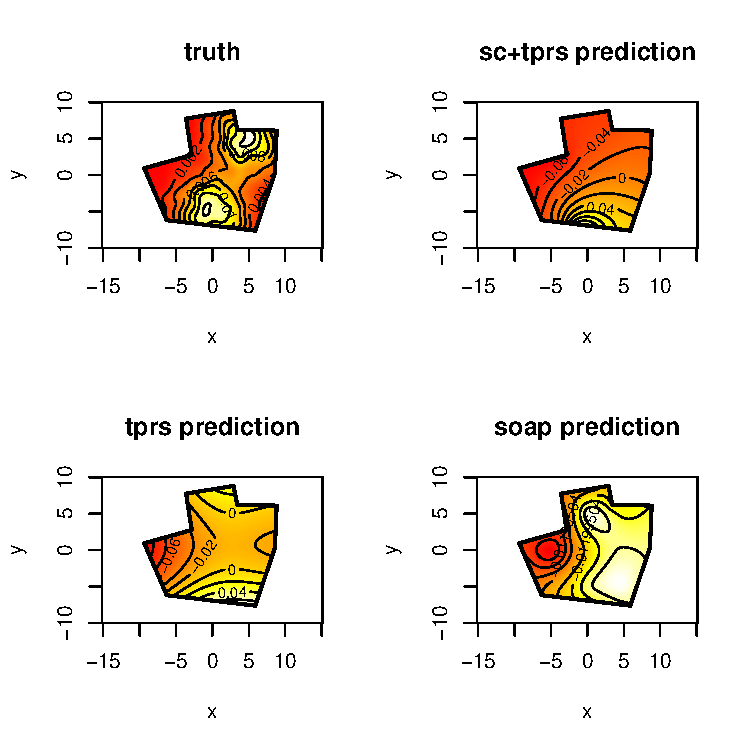
\includegraphics[width=2.5in]{figs-otherdomains/fig9-high-rect.png} \\
\caption{high rect}
\label{fig9-high-rect}
\end{figure}

\begin{figure}
\centering
% trim order l b r t
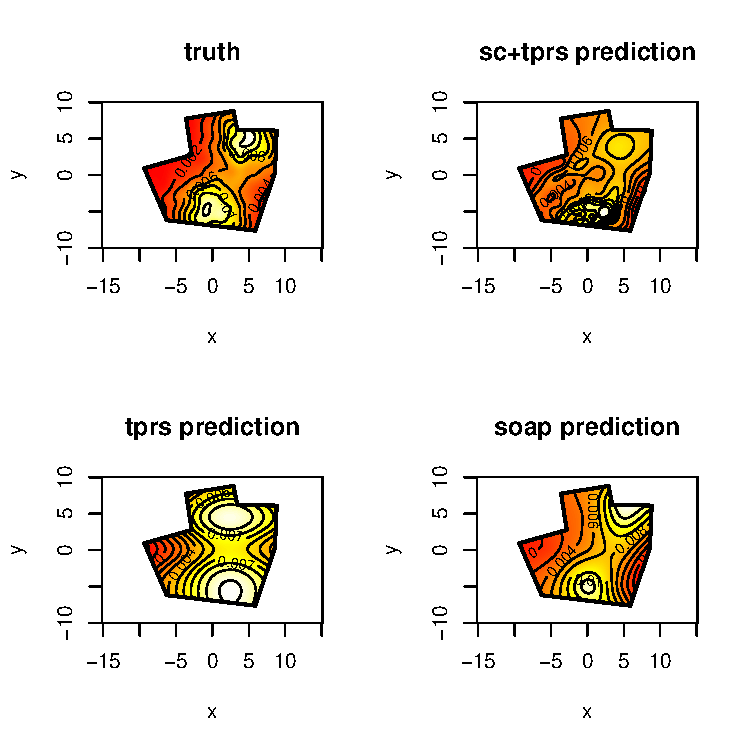
\includegraphics[width=2.5in]{figs-otherdomains/fig9-low-disk.png} \\
\caption{low disk}
\label{fig9-low-disk}
\end{figure}

\begin{figure}
\centering
% trim order l b r t
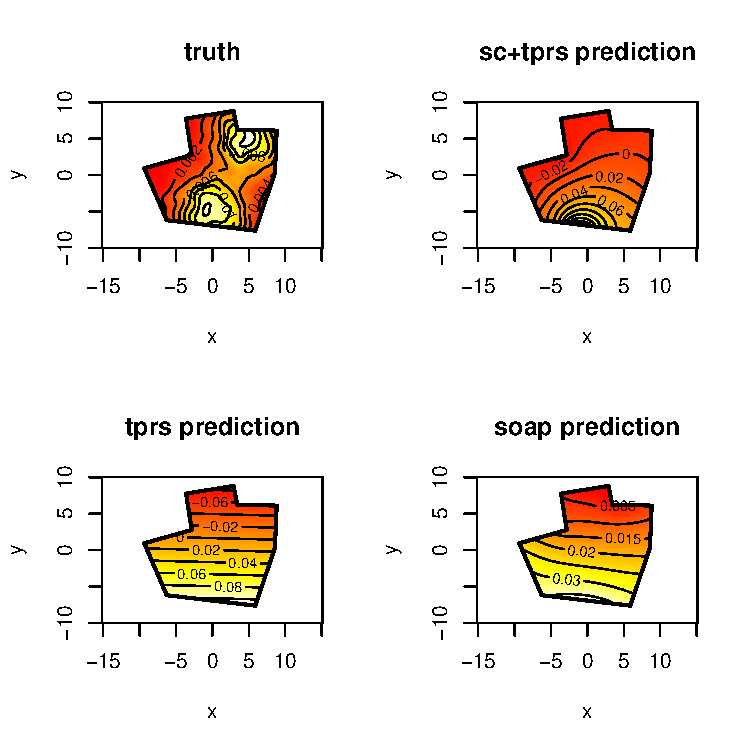
\includegraphics[width=2.5in]{figs-otherdomains/fig9-high-disk.png} \\
\caption{high disk}
\label{fig9-high-disk}
\end{figure}


\section{Wigglytop}


Blahblah blah what is it etc

In our initial simulations, we picked 10,000 from 250,000 points generated over the shape. We then added Normal noise ($\sigma^2=0.02$.) In this domain it would seem that picking the vertices to amap to the corners of the rectangle is crucial.

In the first attempt the SC Toolbox was allowed to pick the corners automatically using the \texttt{crrectmap} routine, this routine also uses the CRDT algorithm to increase the numerical stability of the solution. \Fig{wigglyfirstcomp} shows the comparison between the truth, the \sch transform with thin plate regression splines and using thin plate regression splines without the transform. The MSE was calculated for both models and there was not a large difference between the two. The thin plate method reported an MSE of 9.221594e-05 while using the transform reported 9.154827e-05. Although the difference is very small, it is obvious from looking at the heatmaps that something has gone wrong.

\begin{figure}
\centering
% trim order l b r t
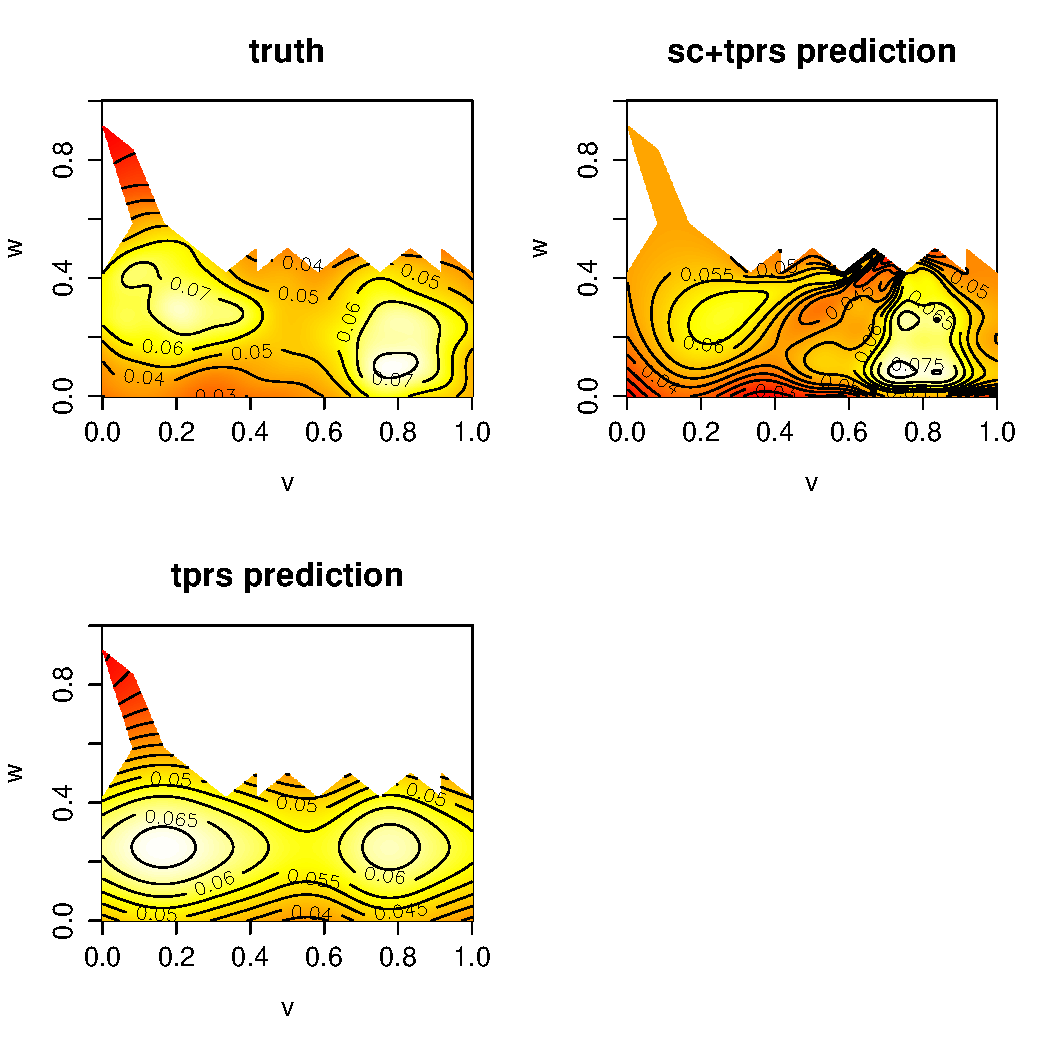
\includegraphics[width=3in]{figs-otherdomains/wigglytop-first.png} \\
\caption{Clockwise from top left: truth, the fit from the transformation method and the fit from a standard thin plate regression spline. The transform is when \texttt{crrectmap} is allowed to choose the vertices to map to the corners of the rectangle.}
\label{wigglyfirstcomp}
% generated by /phd-smoothing/wigglytop/fit...
\end{figure}

To investigate this, the vertices that are to be mapped to the corners were selected manually, still using \texttt{crrectmap}. 

sc+tprs 6.043222e-05 
tprs 9.157006e-05 

\begin{figure}
\centering
% trim order l b r t
\includegraphics[width=2in]{figs-otherdomains/wigglytop-numbered.png} \\
\caption{}
\label{wigglynumbered}
% generated by /phd-smoothing/wigglytop/fit...
\end{figure}

\begin{figure}
\centering
% trim order l b r t
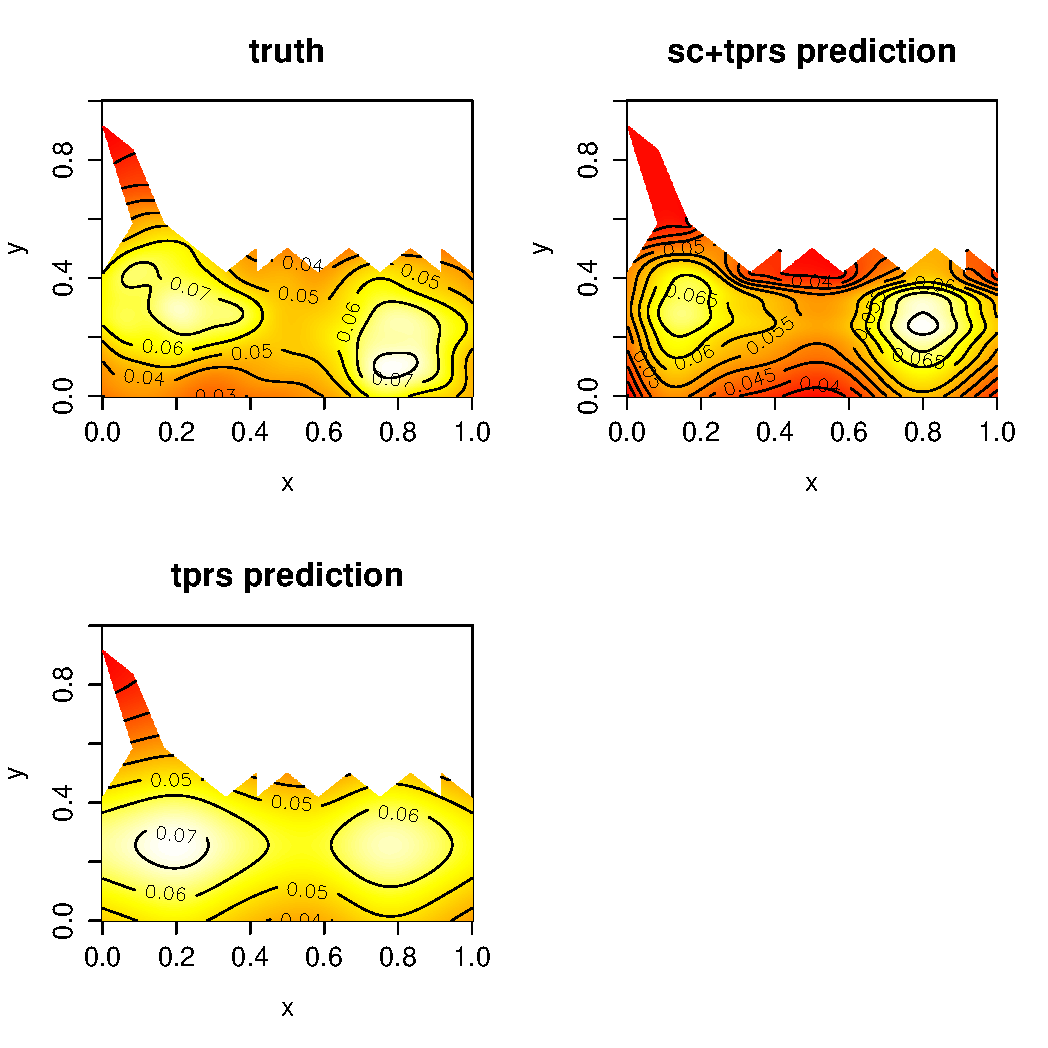
\includegraphics[width=3in]{figs-otherdomains/wigglytop-second.png} \\
\caption{Clockwise from top left: truth, the fit from the transformation method and the fit from a standard thin plate regression spline. The transform is when vertices to map to corners are specified manually.}
\label{wigglyseccomp}
% generated by /phd-smoothing/wigglytop/fit...
\end{figure}




this is just using rectmap
Second try, as before but with the real corners selected
sc+tprs 7.358453e-05 
tprs 9.51009e-05 




\section{Wigglytop2}

We repeated the procedure for another polygon with two peninsulae, shown in \fig{wigglytop2dia}. Initially, a transform using \texttt{rectmap} was used, but this failed to converge, so \texttt{crrectmap} was used.



\begin{figure}
\centering
% trim order l b r t
\includegraphics[width=3in]{figs-otherdomains/wigglytop2dia.png} \\
\caption{}
\label{wigglytop2dia}
% generated by /phd-smoothing/wigglytop/fit...
\end{figure}




With bounding box, first try using the suggested vertices, 
sc+tprs 0.01665045 
tprs 0.02670411 


Then picking the two points inbetween the peninsulae and the two "corners"

sc+tprs 0.02512868 
tprs 0.02666584 


Using a different two vertices:

sc+tprs 0.01756846 
tprs 0.02675054 


\bibliographystyle{plainnat}
\bibliography{sc-refs}



\end{document}
